\documentclass[a4paper,usenatbib]{aspdoc}
\usepackage{newtxtext,newtxmath}
\usepackage{ae,aecompl}
\usepackage{graphicx}	% Including figure files
\usepackage{amsmath}	% Advanced maths commands
\usepackage{amssymb}	% Extra maths symbols
\usepackage{lipsum}
\usepackage{float}
\usepackage{multirow}
\usepackage{booktabs}
\usepackage{geometry}
\usepackage{bm}
\usepackage[load=prefixed]{siunitx}
\sisetup{output-decimal-marker = {,}}
\geometry{left=25mm,right=25mm,top=25mm,bottom=25mm}

\newcounter{simplecount}
\setcounter{simplecount}{0}
\renewcommand{\theequation}{\arabic{simplecount}}
\newcommand{\owncount}{\refstepcounter{simplecount}}

% Title
\title[]{BRZ: Brennstoffzelle}

% The list of authors
\author[]{
    Riedel Lisa, Wegmann Peter
    \newauthor
    \,Gruppe 6
}
% Don't change these lines
\begin{document}
    \label{firstpage}
    \pagerange{\pageref{firstpage}--\pageref{lastpage}}
    \maketitle
    
    

    % Body
    \section{Einleitung}\label{sec:intro}
            Dieser Versuch kann in zwei Teile gegliedert werden.\\
            Im ersten Teil wurden die Eigenschaften des Elektrolyseurs bestimmt.
            Im zweiten Teil wurde der Wirkungsgrad der Brennstoffzelle und deren Kennlinien in Parallel- und Reihenschaltung mit verschiedenen Lastwiderständen untersucht.

                
    
    \section{Verwendete Methoden}\label{sec:method}
        \subsection{Wirkungsgrad}
            In Kapitel \ref{subsec:wirkung} werden die zwei unterschiedlichen Wirkungsgrade $\varepsilon_{\mathrm{E}}$ und $\varepsilon_{\mathrm{F}}$ berechnet. Bei $\varepsilon_{\mathrm{E}}$ handelt es sich um den Faraday-Wirkungsgrad, bei $\varepsilon_{\mathrm{F}}$ um den Energiewirkungsgrad. Im folgenden werden die Formeln zur Berechnung dieser Wirkungsgrade, sowohl für den Elektrolyseur als auch der Brennstoffzelle, beschrieben.
            Bei beiden berechnet sich die theoretische Änderung des erwarteten Wasserstoffvolumen wie folgt.
            \begin{equation}
                \owncount
                \dot{V}_{\mathrm{H_2, theo}} = \frac{dV_{\mathrm{H2, theo}}}{dt} = \frac{I\cdot V_{\mathrm{m}}}{z\cdot F}
                \label{eq:volumen_theo}
            \end{equation}
            Hierbei ist $I$ der elektrische Strom, $F = $ \SI{96485}{\frac{C}{mol}} die Faradaykonstante, $z = 2$ die durchtretenden Elektronen, sowie $V_{\mathrm{m}}$ das molare Gasvolumen.
            \\
            Nun muss noch das molare Gasvolumen berechnet werden. Dies geschieht unter Verwendung folgender Gleichung.
            \begin{equation}
                \owncount
                V_{\mathrm{m}} = \frac{R\cdot T}{p}
                \label{eq:gasvol}
            \end{equation}
            Hierbei ist $R = $ \SI{8,31}{\frac{J}{mol K}} die allgemeine Gaskonstante, $T$ die Temperatur, sowie $p$ der Druck.
            
            \subsubsection{Elektrolyseur}
                Der Elektrolyseur produziert den Wasserstoff. Die Berechnung von $\varepsilon_{\mathrm{F}}$, sowie $\varepsilon_{\mathrm{E}}$ sei wie folgt.
                \begin{equation}
                    \owncount
                    \varepsilon_{\mathrm{F}} = \frac{\dot{V}_{\mathrm{H2, exp}}}{\dot{V}_{\mathrm{H2, theo}}}
                    \label{eq:wirkung_faradayElektro}
                \end{equation}
                \begin{equation}
                    \owncount
                    \varepsilon_{\mathrm{E}} = \frac{\Delta H^0 \cdot N_{H_{2}}}{U\cdot I \cdot t}
                    \label{eq:wirkung_energie}
                \end{equation}
                Die Standardverbrennungsenthalpie $\Delta H^0 = $ \SI{286}{\frac{kJ}{mol}} bezeichnet den chemischen Energiegehalt von $\mathrm{H}_2$, $N_{H_{2}}$ die Stoffmenge von $\mathrm{H}_2$ in mol. 
                Hierbei verwendet man die in Kapitel \ref{subsec:wirkung} aufgeführten Werte, für das jeweilige betrachtete Bauteil.
            
            \subsubsection{Brennstoffzelle}
                Im Unterschied zum Elektrolyseur, erzeugt die Brennstoffzelle keinen Wasserstoff, sondern verbraucht ihn. Somit muss für $\varepsilon_{\mathrm{F}}$ der Kehrwert gebildet werden.
                \begin{equation}
                    \owncount
                    \varepsilon_{\mathrm{F}} = \frac{\dot{V}_{\mathrm{H2, theo}}}{\dot{V}_{\mathrm{H2, Exp}}}
                    \label{eq:wirkung_faradayBrenn}
                \end{equation}
                Die Berechnung von $\varepsilon_{\mathrm{E}}$ erfolgt durch Bildung des Kehrwertes von Gleichung \ref{eq:wirkung_energie}.
                \begin{equation}
                    \owncount
                    \varepsilon_{\mathrm{E}} = \frac{U\cdot I \cdot t}{\Delta H^0 \cdot N_{H_{2}}}
                    \label{eq:wirkung_energieBrenn}
                \end{equation}
                \\
                Die Berechnung von $\varepsilon_{\mathrm{F}}$ und $\varepsilon_{\mathrm{E}}$ erfolgt anschließend durch einsetzten der in Kapitel \ref{subsec:wirkung} aufgeführten Werte.
    
        % Figures moved up from chapter "Leckrate"
            \begin{figure*}
                \centering
                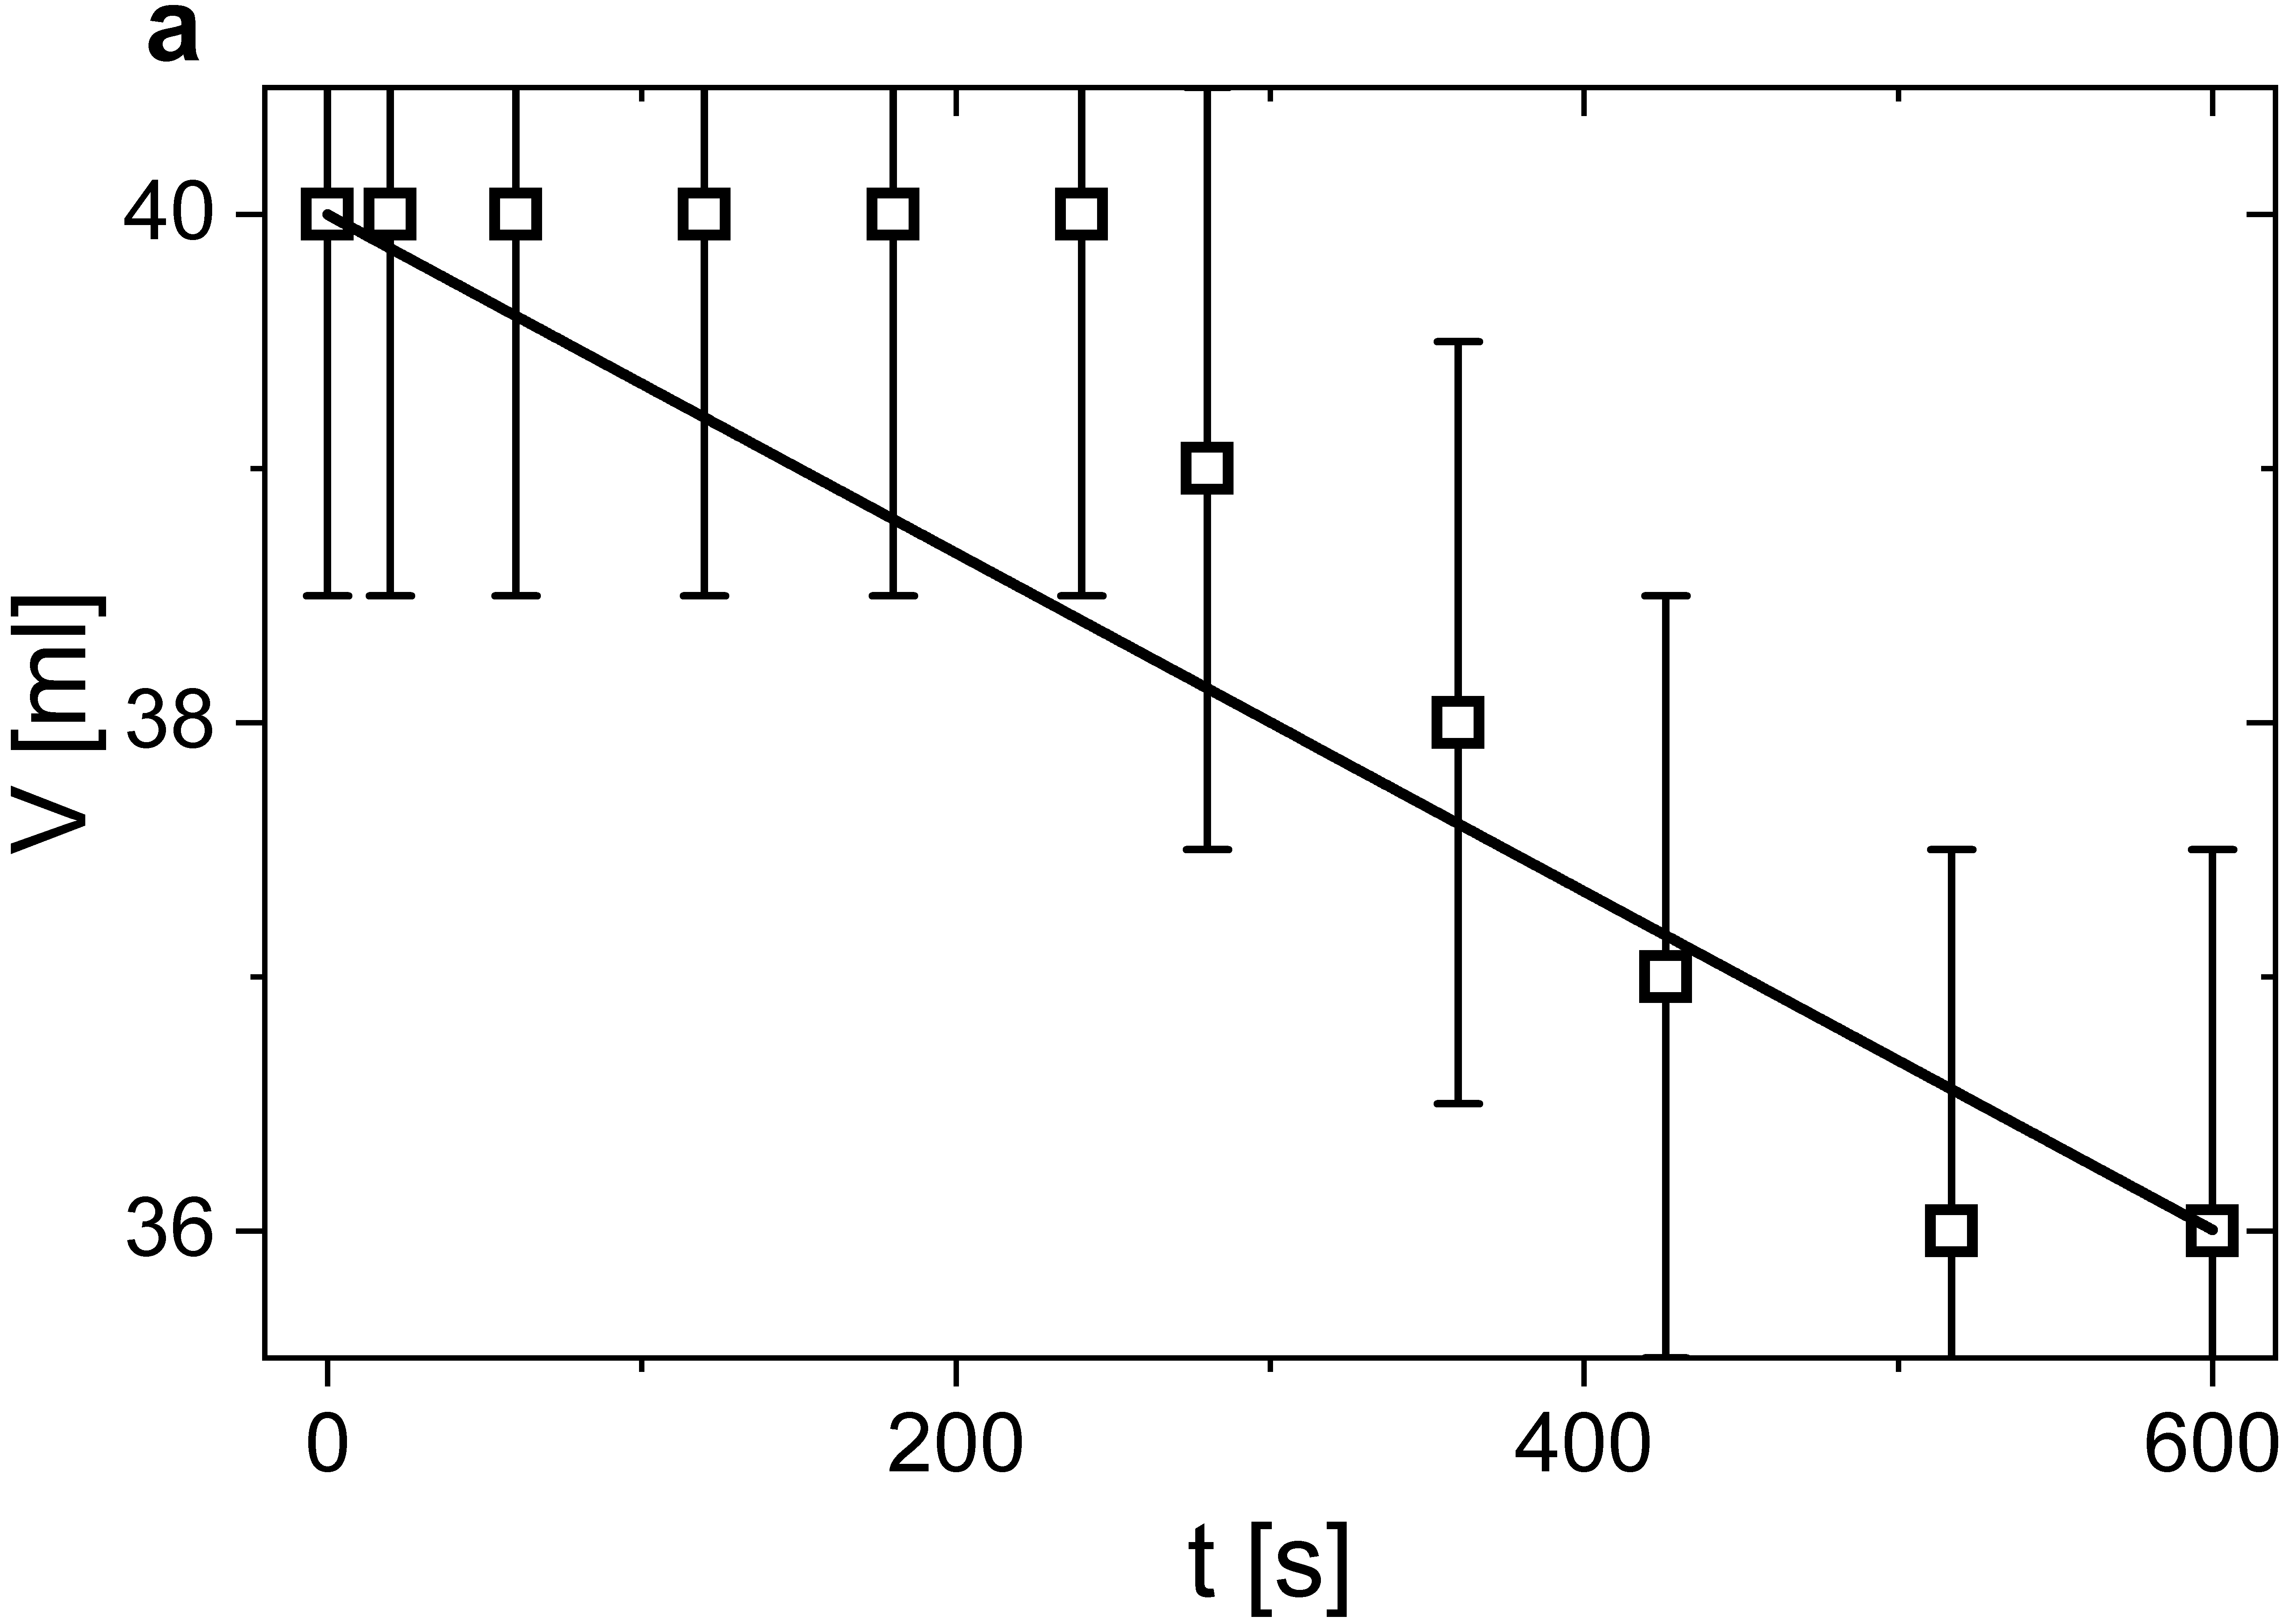
\includegraphics[width=78mm]{graphs/leck1.png}
                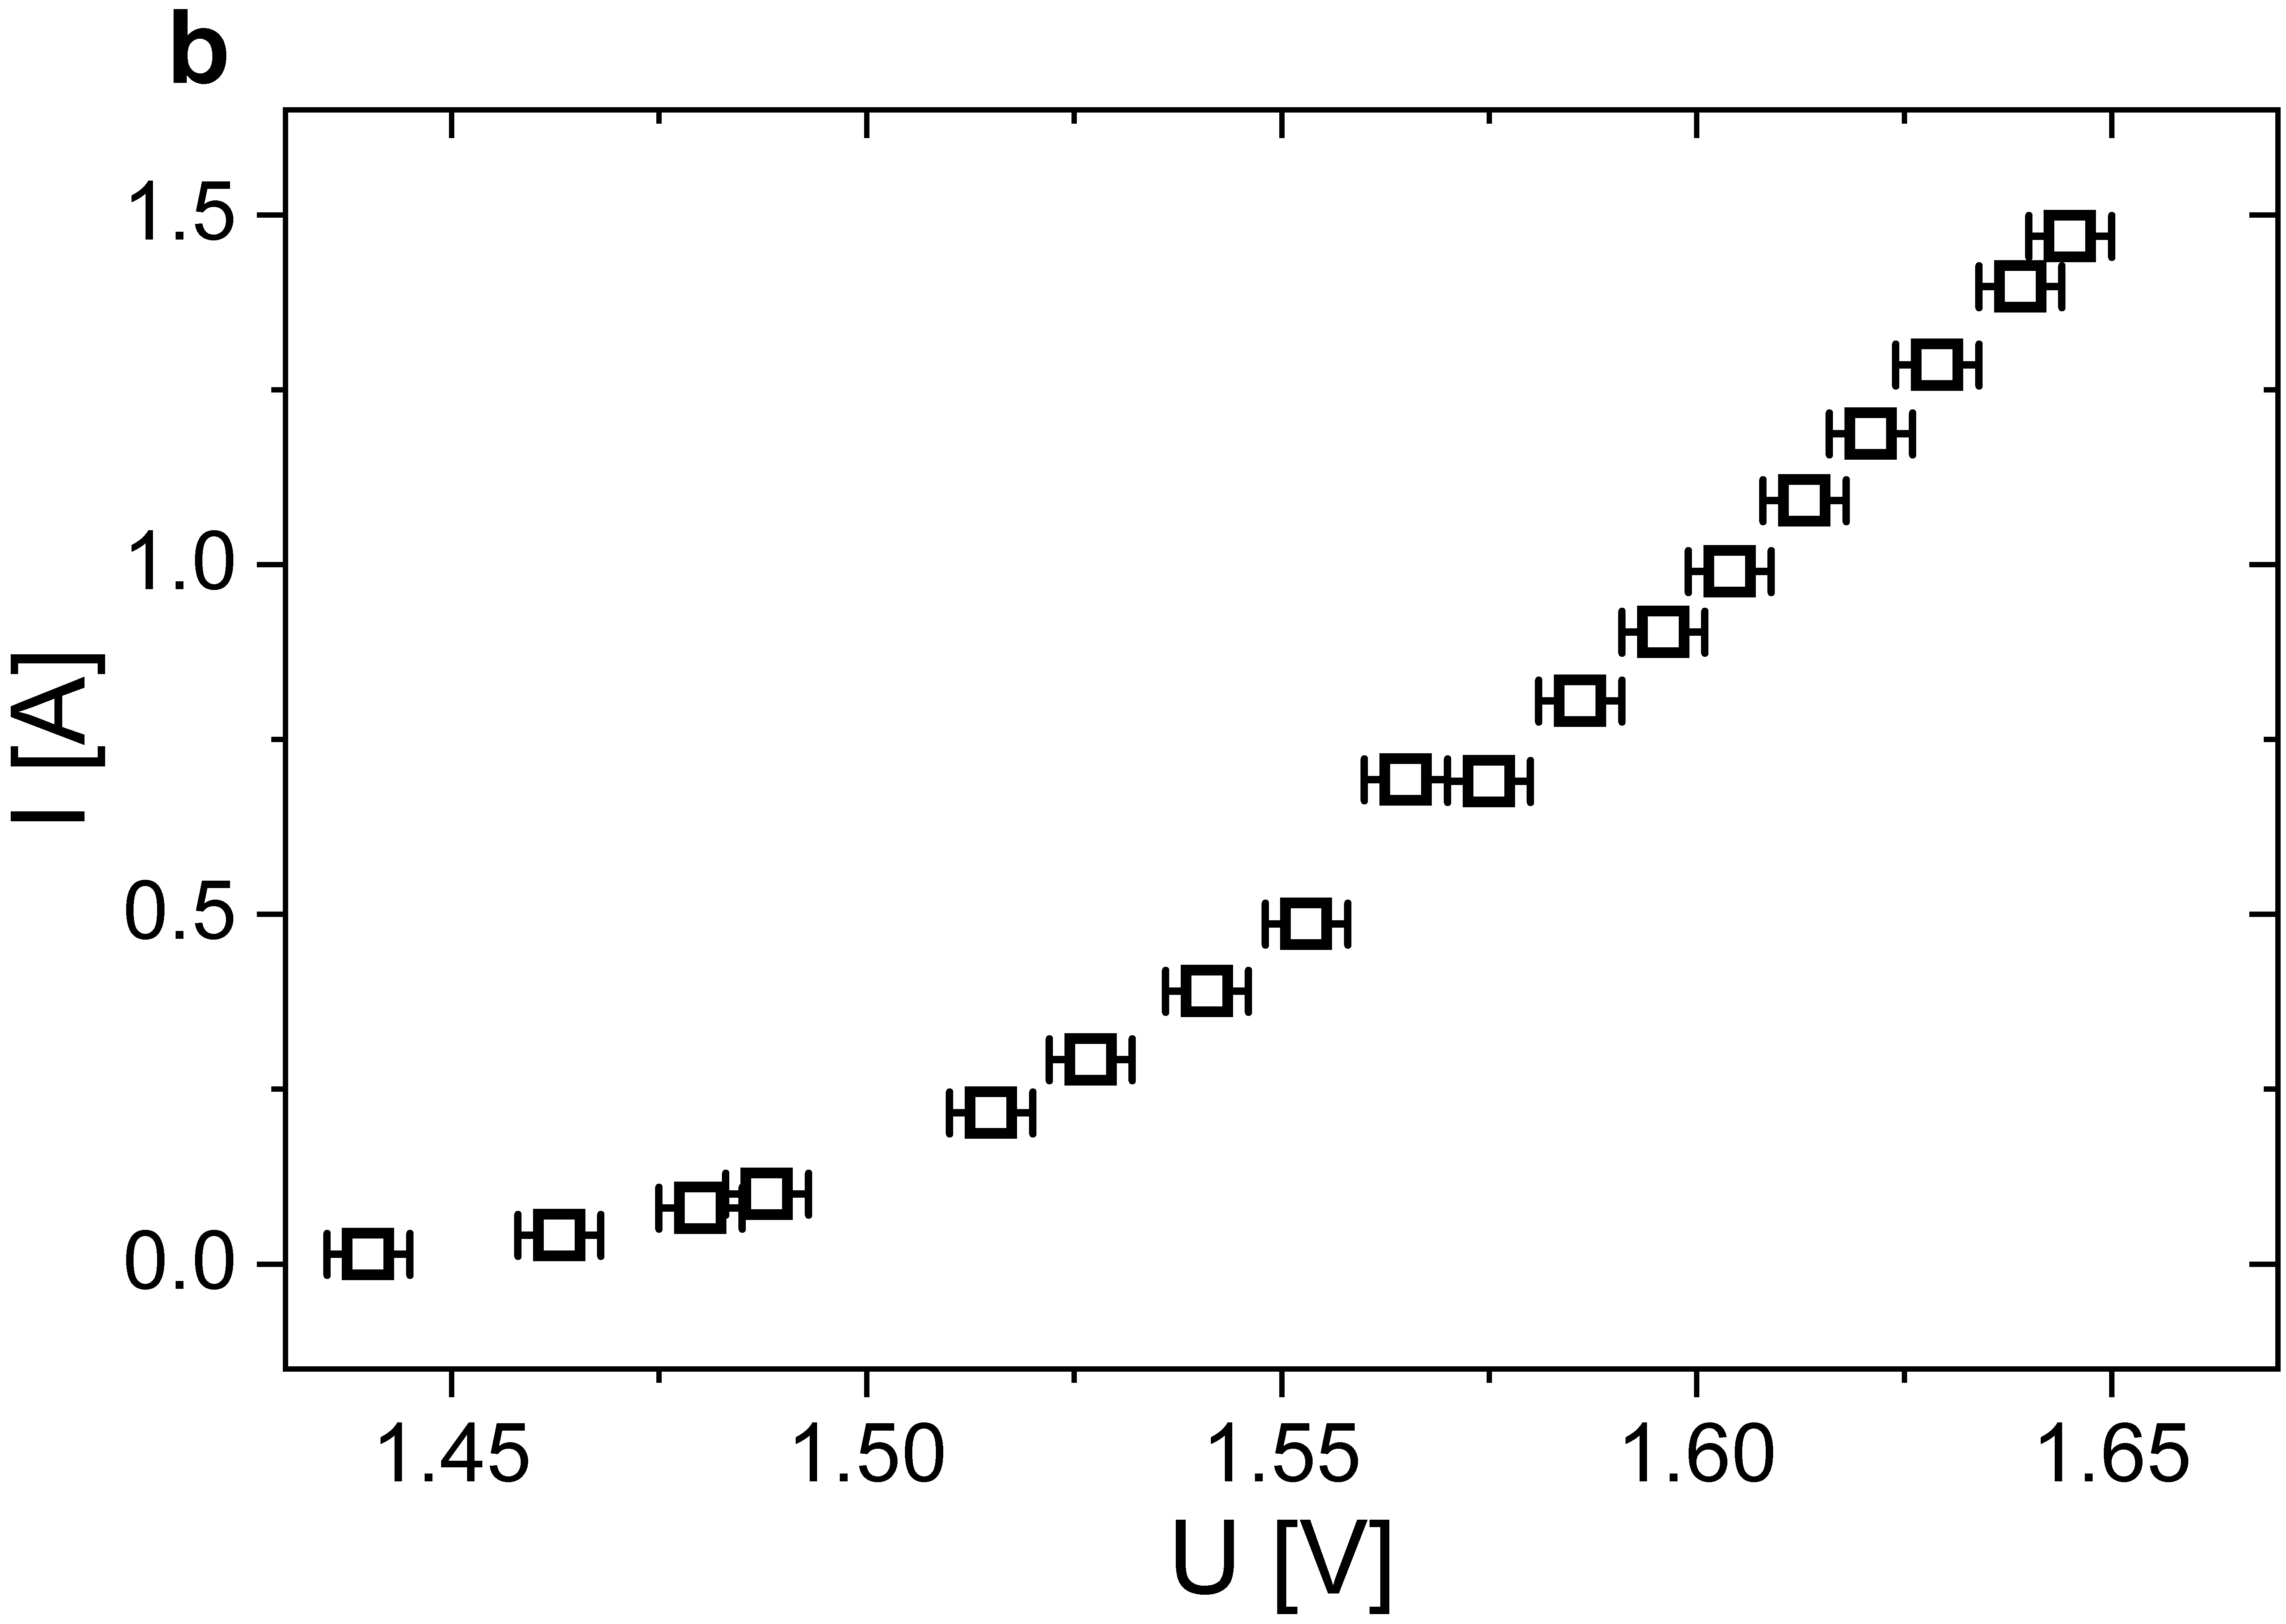
\includegraphics[width=78mm]{graphs/elekChar1.png}
                \caption{
                    \textbf{a} Wasserstoffvolumen $V$ in Relation zur Zeit. Die Steigung der Ausgleichsgerade stellt die Leckrate dar. Die dargestellte Ausgleichsgerade besitzt eine Steigung von 6,6$\cdot 10^{-3} \frac{\mathrm{ml}}{\mathrm{s}}$, was auf eine Leckrate von \SI{3,9}{\frac{\milli\litre}{min}} schließen lässt.
                    \textbf{b} Kennlinie des Elektrolyseurs. Die anfänglich geringe Steigung der Kennlinie stellt ein langsamen einsetzten des Stromflusses dar. Wird eine gewisse Spannung überschritten, ist ein linearer Zusammenhang zwischen Strom und Spannung erkennbar.
                }
                \label{fig:leckRate}
            \end{figure*}
            
        
        \subsection{Charakterisierung der Elektrochemischen Zelle}
            Im folgenden werden verwendete Gleichungen zur Berechnung des  Durchtrittsfaktor $\alpha$ und Austauschstromstärke $I_0$ aufgeführt.
            \\
            Hierfür berechnet man zuerst die Durchtrittsüberspannung $\eta_{\mathrm{Durch}}$ mittels folgender Gleichung.
            \begin{equation}
                \owncount
                \begin{aligned}
                    U = E_0 - \eta_{\mathrm{Durch}} - \eta_{\mathrm{Ohm}} - \eta_{\mathrm{Diff}} \Leftrightarrow \\
                    \eta_{\mathrm{Durch}} = E_0 - I\cdot R_{\mathrm{Innen}} - U - \eta_{\mathrm{Diff}}
                \end{aligned}
                \label{eq:etaDurch}
            \end{equation}
            mit $E_0 = 1,23$ V als theoretisch mögliche Spannung mit offenen Lastwiderstand, $U$ und $I$ als jeweils gemessene Spannung und Strom, sowie $R_{\mathrm{Innen}}$ als berechneten Innenwiderstand. Da $\eta_{\mathrm{Durch}}$ später lediglich im elektrokinetischen Bereich betrachtet wird, kann $\eta_{\mathrm{Diff}} \approx 0$ genähert werden.
            \\
            Die konkrete Berechnung von $\alpha$ und $I_0$ geschieht unter Verwendung der Tafelgleichung.
            \begin{equation}
                \owncount
                \eta_{\mathrm{Durch}} = \frac{RT}{(1-\alpha)z\cdot F} \ln\left(\frac{I}{-I_0}\right)
                \label{eq:tafelFit}
            \end{equation}
            Diese Gleichung wird in Kapitel \ref{subsec:char_zel} in Abbildung \ref{fig:brennVerbrauchRate}b gefittet. Durch diesen Fit lassen sich anschließend die gesuchten Größen durch die folgende, konkrete Gleichung finden.
            \begin{equation}
                \owncount
                \eta_{\mathrm{Durch}} = s\cdot \ln(I) - b
                \label{eq:fit}
            \end{equation}
            Die gesuchten Größen sind somit $s$ und $b$.
            \\
            Nun lässt sich $\alpha$ durch Umstellen von Gleichung \ref{eq:tafelFit} und Gleichung \ref{eq:durchtrittsfaktor} berechnen.
            \begin{equation}
                \owncount
                s = \frac{RT}{F\,z \,(1- \alpha)}
                \label{eq:durchtrittsfaktor}
            \end{equation}
            Die Berechnung von $I_0$ geschieht under Verwendung von Gleichung \ref{eq:fit}.
            \begin{equation}
                \owncount
                v = s \,\ln(-I_0)
                \label{eq:austauschstrom}
            \end{equation}

       
    
    \section{Experimentelles Vorgehen}\label{sec:experiment}
        Zur Bestimmung der Leckrate des Elektrolyseurs wurde ein Gasvolumen von \SI{30}{\milli\litre} erzeugt. Danach wurden die elektrischen Verbindungen getrennt, und der Füllstand des Wasserreservoirs über 10 Minuten gemessen. Der Füllstand wurde an einer Skala mit \SI{2}{\milli\litre} Unterteilung abgelesen.\\
        Damit ein $U-I$-Diagramm des Elektrolyseurs erstellt werden kann, wurde von \SI{0}{\ampere} bis \SI{1,5}{\ampere}, in \SI{0,1}{\ampere}-Schritten, die Spannung und der Strom notiert.\\
        Danach wurde der Wirkunsgrad des Elektrolyseurs zu einem konstanten Strom von \SI{1}{\ampere} und einer konstanten Spannung von \SI{1,605}{\volt} bestimmt. Hierfür wurde über 6 Minuten der Füllstand des Wasserreservoirs gemessen. Die Bestimmung des Wirkungsgrad erfolgte anschließend rechnerisch.\\
        Zur Bestimmung des Wirkungsgrades der Brennstoffzelle wurde diese vorher zwei mal mit Gas gespült. Danach wurde ein Gasvorrat von \SI{40}{\milli\litre} erzeugt, die beiden Brennstoffzellen zu einer Parallelschaltung verbunden und die Stromversorgung des Elektrolyseurs getrennt. Bei einem Lastwiderstand von \SI{0,5}{\ohm}  wurde die Zeit, bis ein Gasvolumen von \SI{30}{\milli\litre} verbraucht wurde, gemessen.\\
        Um die Kennlinie der Brennstoffzelle in Parallelschaltung zu ermitteln, wurde die Zelle zuvor zwei mal mit Gas gespült. Danach wurde ein ausreichendes Gasvolumen erzeugt und zu jedem eingebautem Lastwiderstand der Strom und die Spannung, nachdem sich diese stabilisiert haben, notiert. In dem Versuchsaufbau sind 10 Lastwiderstände von \SI{100}{\ohm}, \SI{50}{\ohm}, \SI{20}{\ohm}, \SI{10}{\ohm}, \SI{5}{\ohm}, \SI{3}{\ohm}, \SI{2}{\ohm}, \SI{1}{\ohm}, \SI{0,5}{\ohm}, und \SI{0,3}{\ohm} verbaut. Insgesamt wurden drei Messreihen durchgeführt.\\
        Die Kennlinie in Reihenschaltung wurde identisch zur Parallelschaltung durchgeführt. Die Brennstoffzellen sind mit dem Lastwiderstand in Reihenschaltung verbaut. Es wurden ebenfalls drei Messreihen durchgeführt.
        \\
        In den folgenden Ergebnissen wurde eine konstante Temperatur $T = 296$ K und Druck $p = 960$ hPa angenommen.

        
            
    \section{Ergebnisse}\label{sec:result}
        % Figures moved up from chapter "Wirkungsgrade"
            \begin{figure*}
                \centering
                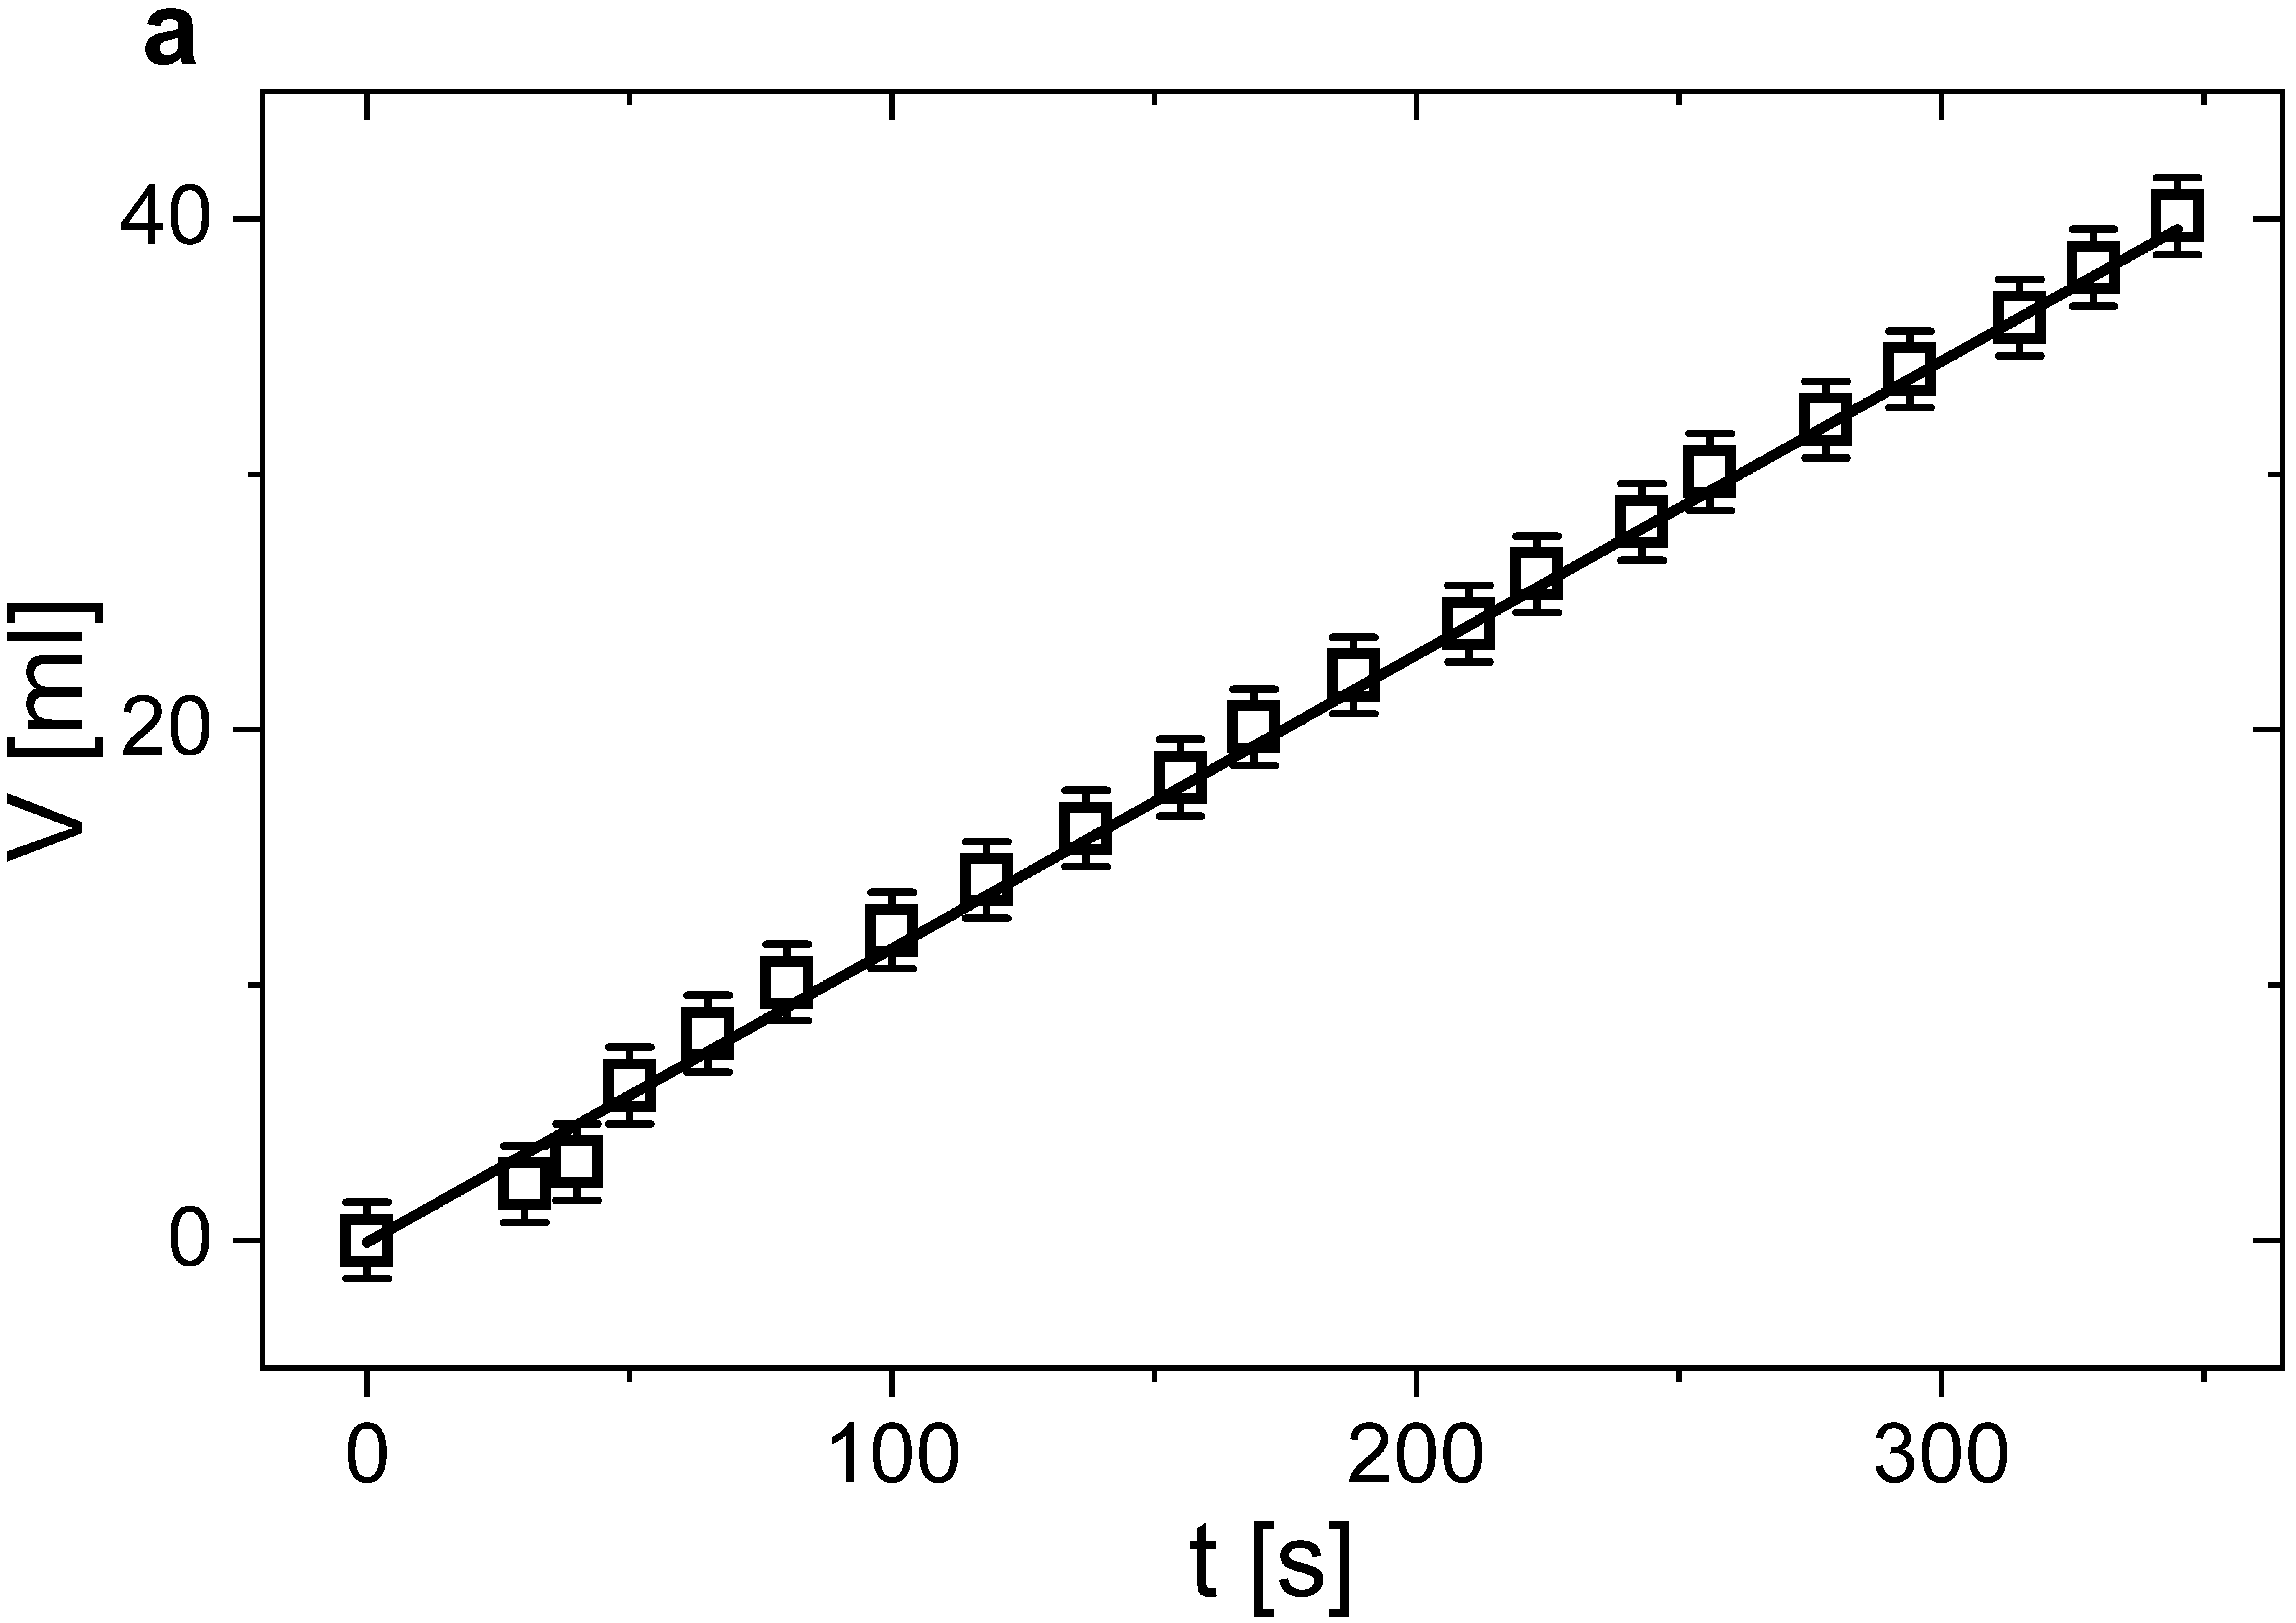
\includegraphics[width=78mm]{graphs/elekWirkung1.png}
                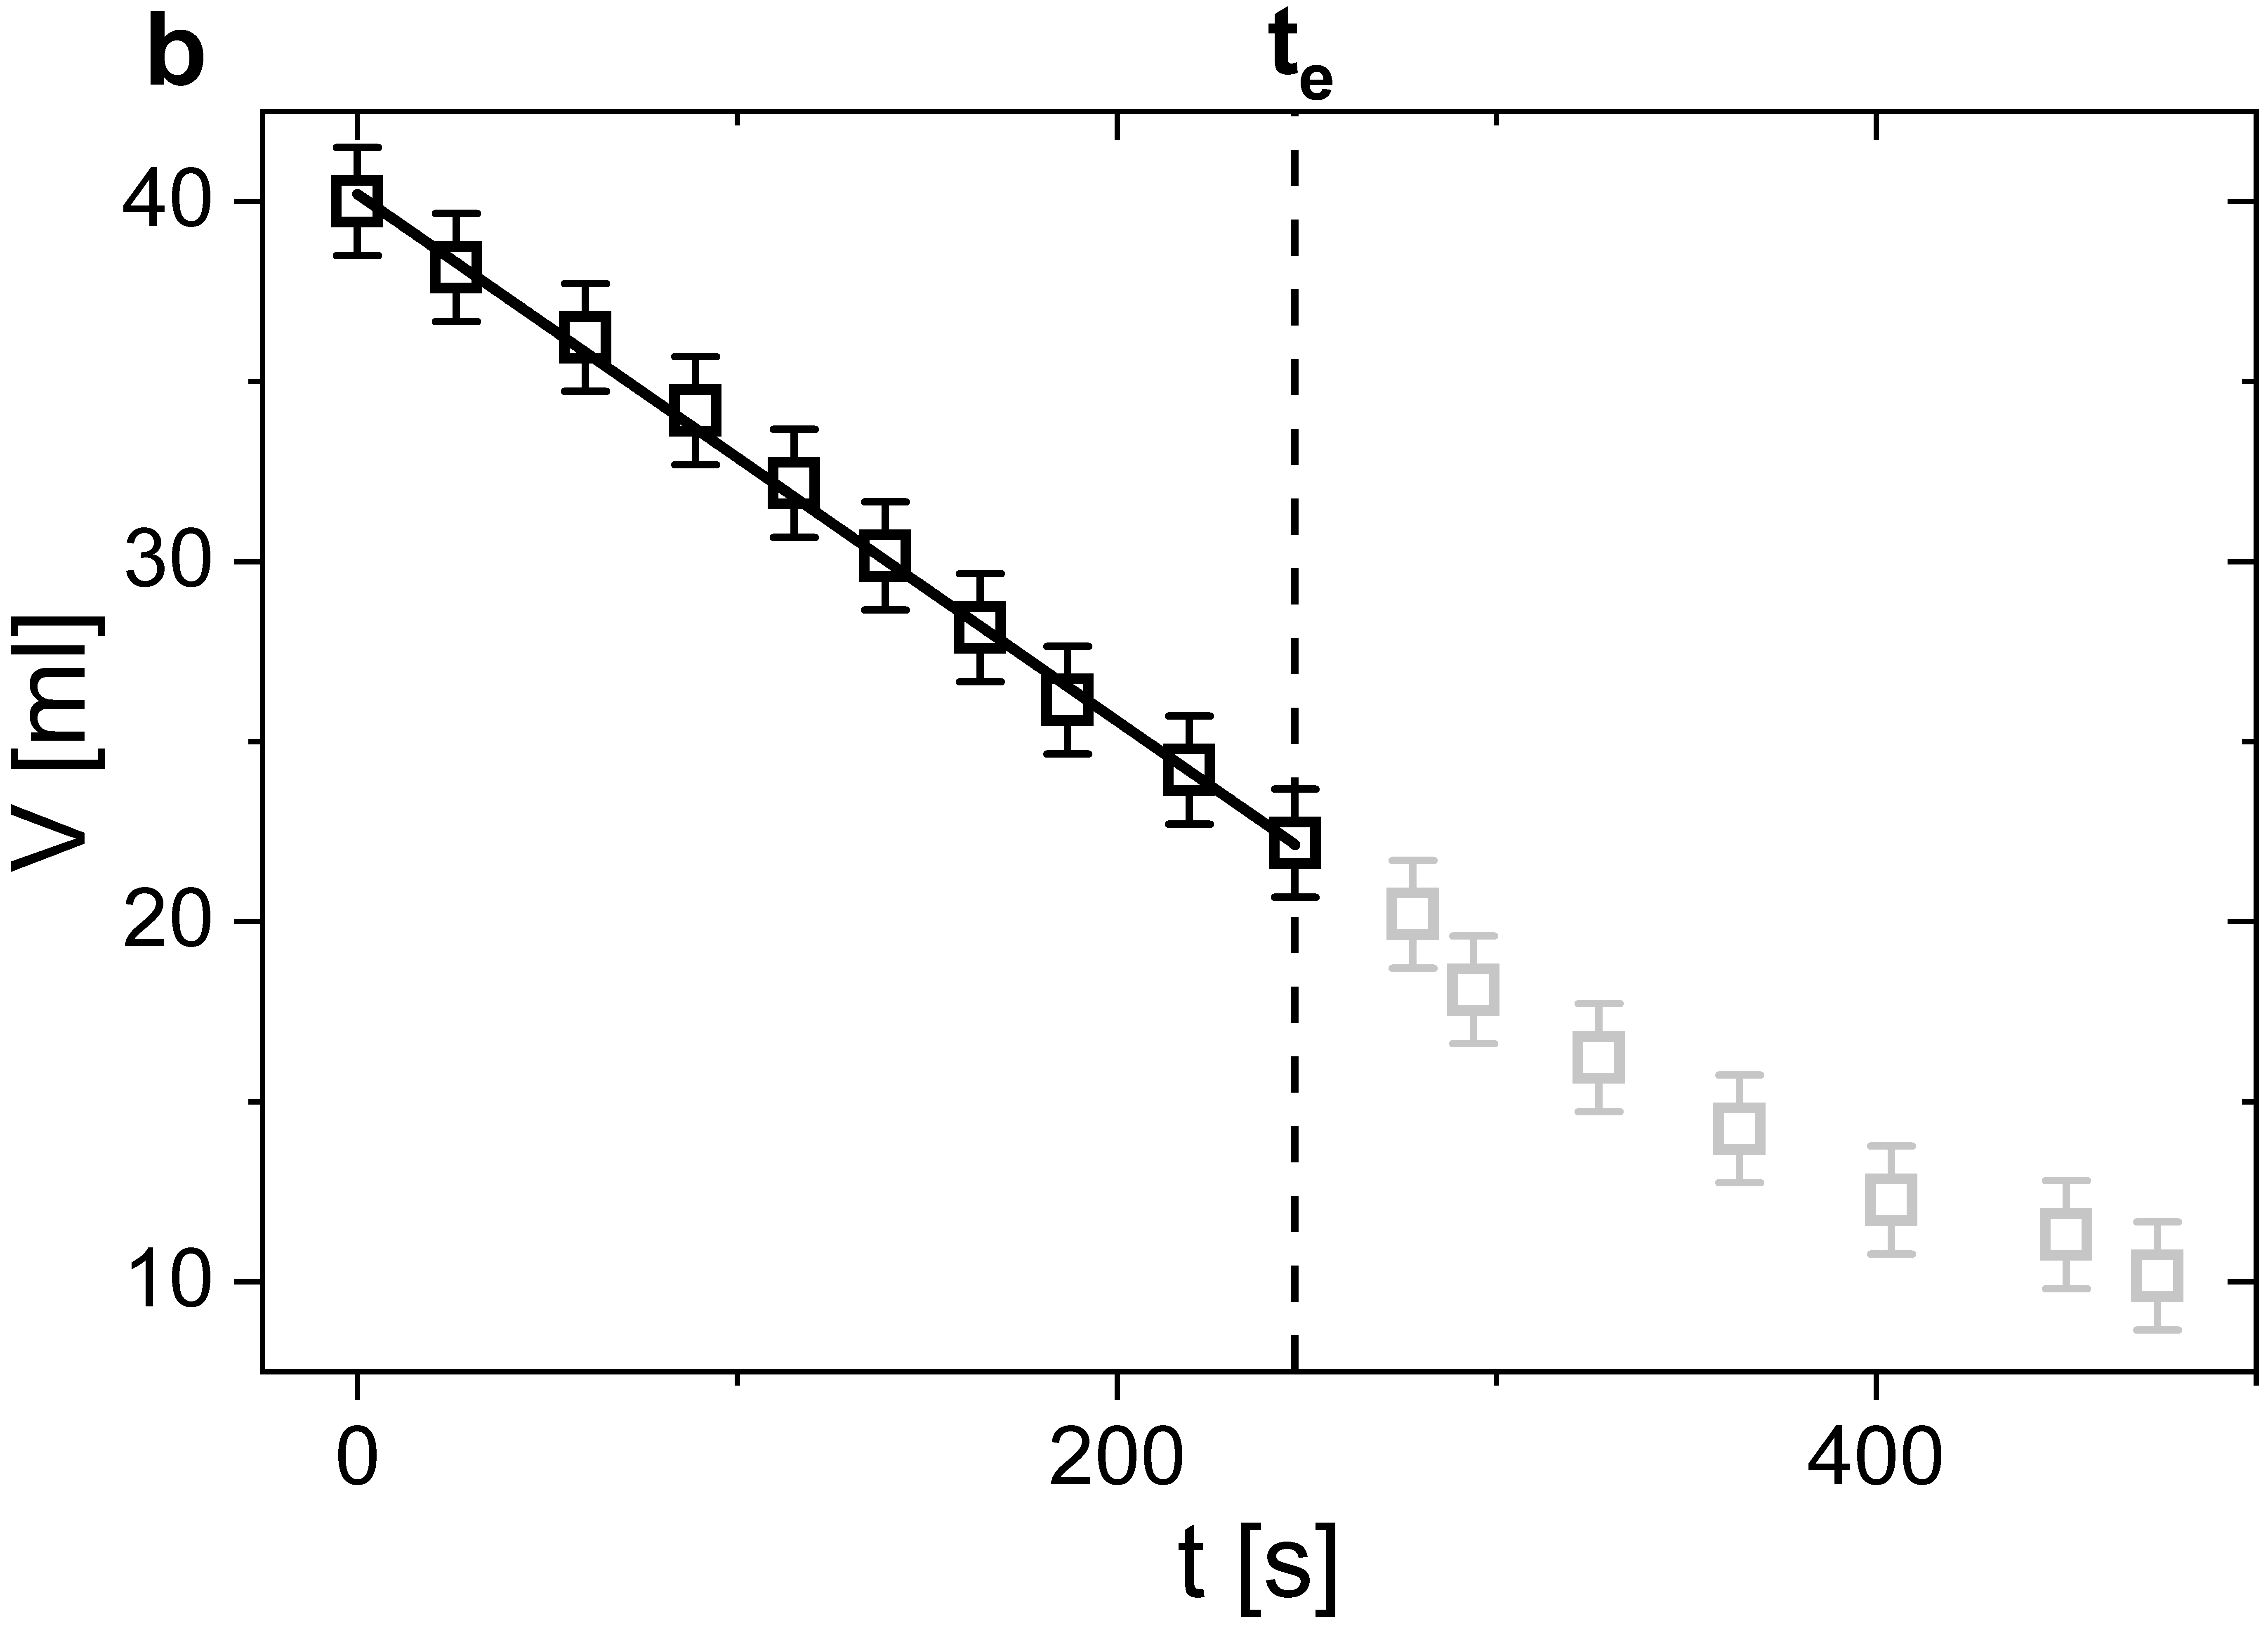
\includegraphics[width=78mm]{graphs/brennWirkung1.png}
                \caption{
                    \textbf{a} Gaserzeugungsrate des Elektrolyseur. Zu sehen ist das erzeugte Gasvolumen $V$ in Abhängigkeit der Zeit. Die Steigung der Ausgleichsgerade beträgt \SI{0,11}{\frac{\milli\litre}{s}}. Dies ergibt eine Erzeugungsrate von \SI{6,89}{\frac{\milli\litre}{min}}.
                    \textbf{b} Wasserstoff-Verbrauchsrate einer Brennstoffzelle bei eine Widerstand von \SI{0,5}{\ohm}. Die Steigung der Ausgleichsgerade beträgt \SI{0,07}{\frac{\milli\litre}{s}}. Dies ergibt eine Verbrauchsrate von \SI{4,38}{\frac{\milli\litre}{min}}. Bei $t_e$ ist der Strom, aufgrund von Wasseransammlungen in der Brennstoffzelle, zusammengebrochen. Diese Werte wurden für die Ausgleichsgerade nicht betrachtet.
                }
                \label{fig:rate}
            \end{figure*}
    
        \subsection{Leckrate}\label{subsec:leck}
            Die Verbindung des Elektrolyseurs und der Brennstoffzelle wurde durch Verbindungsröhre realisiert. Da diese nicht vollkommen Dicht sind, muss die Leckrate bestimmt werden. Hierbei handelt es sich um die Rate von austretendem und diffundierendem Wasserstoff durch die Anschlüsse und Verbindungsröhre. Die Leckrate ist in Abbildung \ref{fig:leckRate} mittels Ausgleichsgerade dargestellt. Die Ableseunsicherheit wurde auf etwa \SI{1,5}{\milli\litre} geschätzt. 
            
            
        \subsection{Charakterisierung des Elektrolyseurs}\label{subsec:char_elektro}
            Der Elektrolyseur erzeugt die beiden benötigten Gase. Hierbei ist die Erzeugung dieser stark von der angelegten Spannung und dem fließendem Strom abhängig. Je mehr Strom fließt, desto höher ist die Gaserzeugungsrate des Elektrolyseurs. In Abbildung \ref{fig:leckRate} ist dessen Kennlinie dargestellt. Bevor der Elektrolyseur das Wasser aufspalten kann, wird eine Mindestspannung benötigt. Dies ist am geringen Anstieg der Kennlinie bei $I \approx 0$ erkennbar.  
        
        
        \subsection{Wirkungsgrad}\label{subsec:wirkung}
            Im folgenden betrachte man die Wirkungsgrade sowie die Erzeugungs-/Verbrauchsrate des Elektrolyseurs und der Brennstoffzelle. Beide Raten sind hierbei in Abbildung \ref{fig:rate} dargestellt.
            \\
            Um die Wirkungsgrade des Elektrolyseurs zu bestimmen, ist sowohl $I$ als auch $U$ notwendig. Die Gaserzeugungsrate wurde, wie in Kapitel \ref{sec:experiment} aufgeführt, bei einem Strom $I = 1,00$ A bestimmt. Die Messung der Spannung ergab dabei $U = 1,60$ V. Einsetzten dieser Werte in Gleichung \ref{eq:wirkung_faradayElektro} und Gleichung \ref{eq:wirkung_energie} ergaben die in Tabelle \ref{tab:wirkung} dargestellten Wirkungsgrade.
            Hierbei ist $\dot{V}_{\mathrm{H2, exp}} = $ \SI{0,11}{\frac{ml}{s}} und $\dot{V}_{\mathrm{H2, theo}} = $ \SI{0,13}{\frac{ml}{s}}, sowie $N_{H_{2}} = 1,59 \cdot 10^{-3}$ mol aufgrund von 40 ml Wasserstoff. Da die Daten über einen Zeitraum von 6 Minuten gesammelt wurden, setzt man in Gleichung \ref{eq:wirkung_energie} $t = 360$ s.
            \\ 
            Die Berechnung beider Wirkungsgrade für die Brennstoffzelle erfolgt analog wie für die des Elektrolyseurs. Aufgrund des Verbrauchs der Brennstoffzelle wurden Gleichung \ref{eq:wirkung_faradayBrenn} und Gleichung \ref{eq:wirkung_energieBrenn} verwendet. Da der Strom nach etwa $187$ s zusammenbrach, betrachte man ein verbrauchtes Wasserstoffvolumen von $14$ ml, und dadurch $N_{H_{2}} = 5,5 \cdot 10^{-4}$ mol. Zudem setzte man $I = 0,48$ A, $U = 0,33$ V. Beide letztere Ergebnisse wurden experimentell bestimmt. Die Ergebnisse sind in Tabelle \ref{tab:wirkung} aufgeführt.
            
            \begin{table}
                \centering
                \begin{tabular}{c|c|c}
                    \multicolumn{1}{c}{} & \multicolumn{1}{c|}{$\epsilon_{\mathrm{F}}$} & \multicolumn{1}{c}{$\epsilon_{\mathrm{E}}$}\\
                    \cmidrule(lr){2-2}\cmidrule(lr){3-3}
                    \toprule
                    \textbf{a}  & $(84,62 \pm 10,01)$\,\% & $(78,95 \pm 7,20)$\,\% \\
                    \textbf{b}    & $(91,43 \pm 17,63)$\,\% & $(18,83 \pm 3,76)$\,\% \\
                    \bottomrule
                \end{tabular}
                \caption{Ergebnisse beider Wirkungsgrade \textbf{a} des Elektrolyseurs und \textbf{b} der Brennstoffzelle. Man beachte den jeweils hohen Faraday-Wirkungsgrad, sowie den erwarteten, geringen Energiewirkungsgrad der Brennstoffzelle.}
                \label{tab:wirkung}
            \end{table}
            
            
            % Moved up from chapter "Kennlinie der Brennstoffzelle"
                \begin{figure*}
                    \centering
                    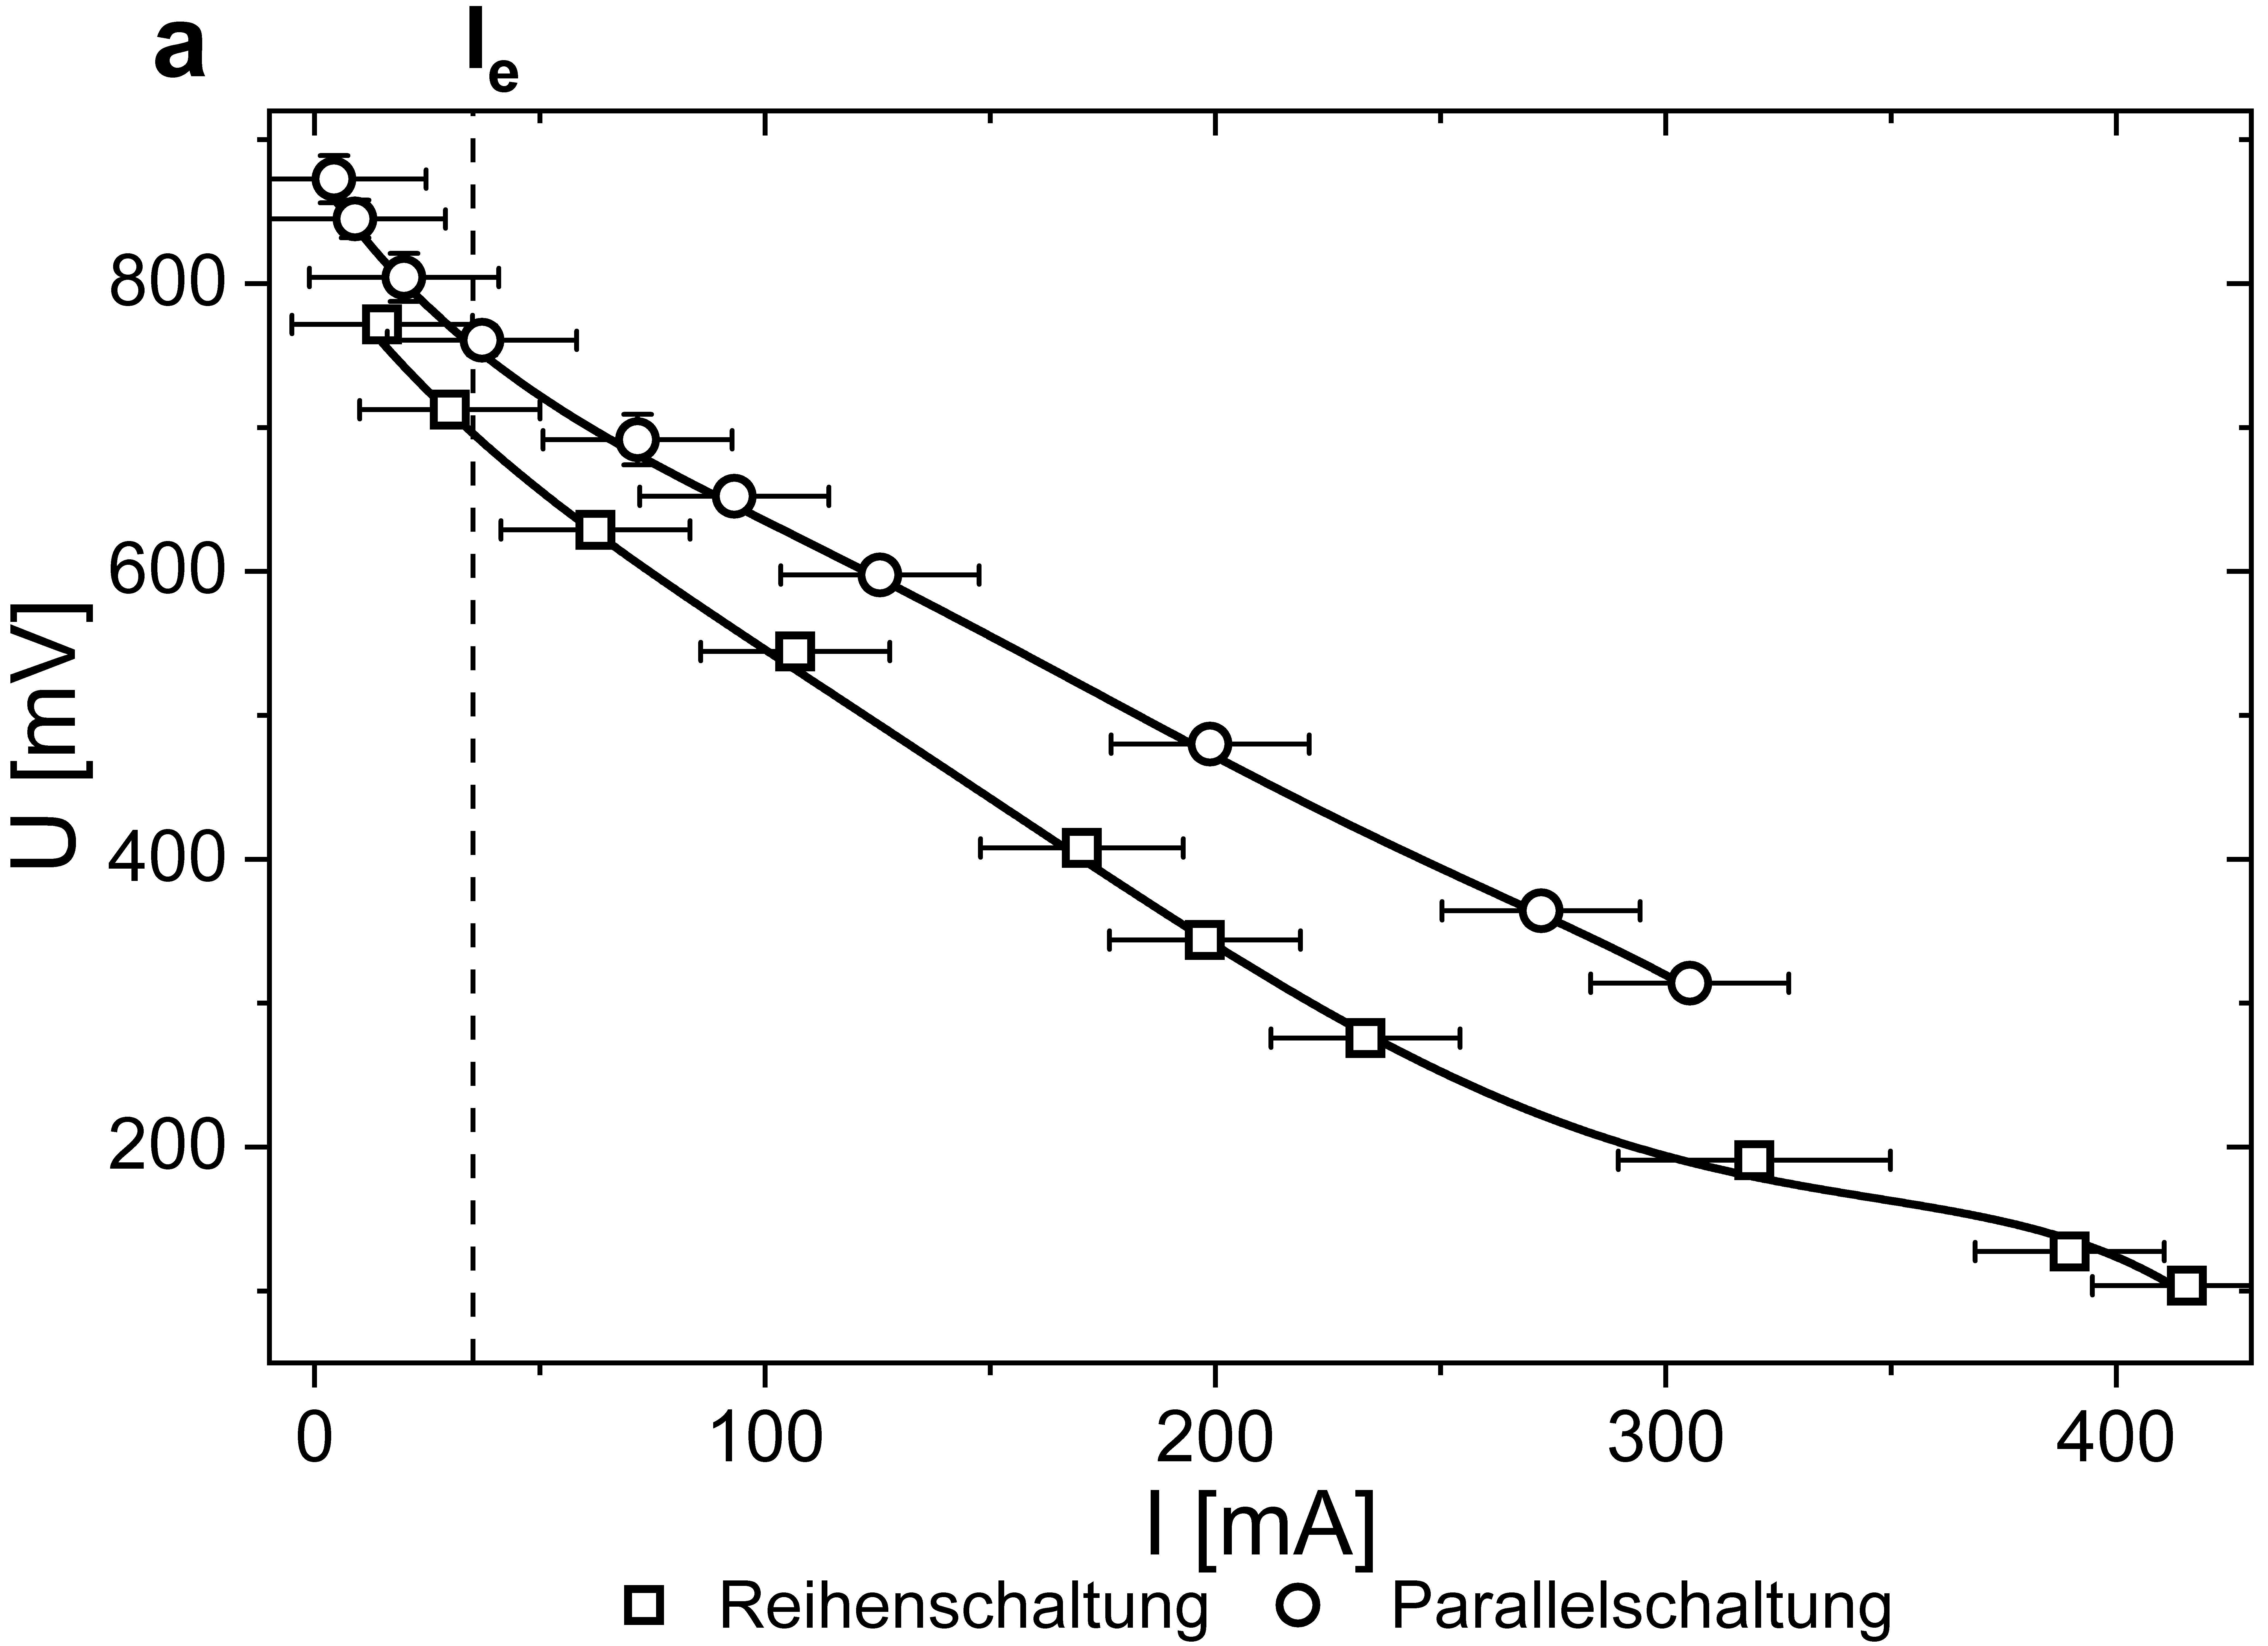
\includegraphics[width=78mm]{graphs/brennKenn1.png}
                    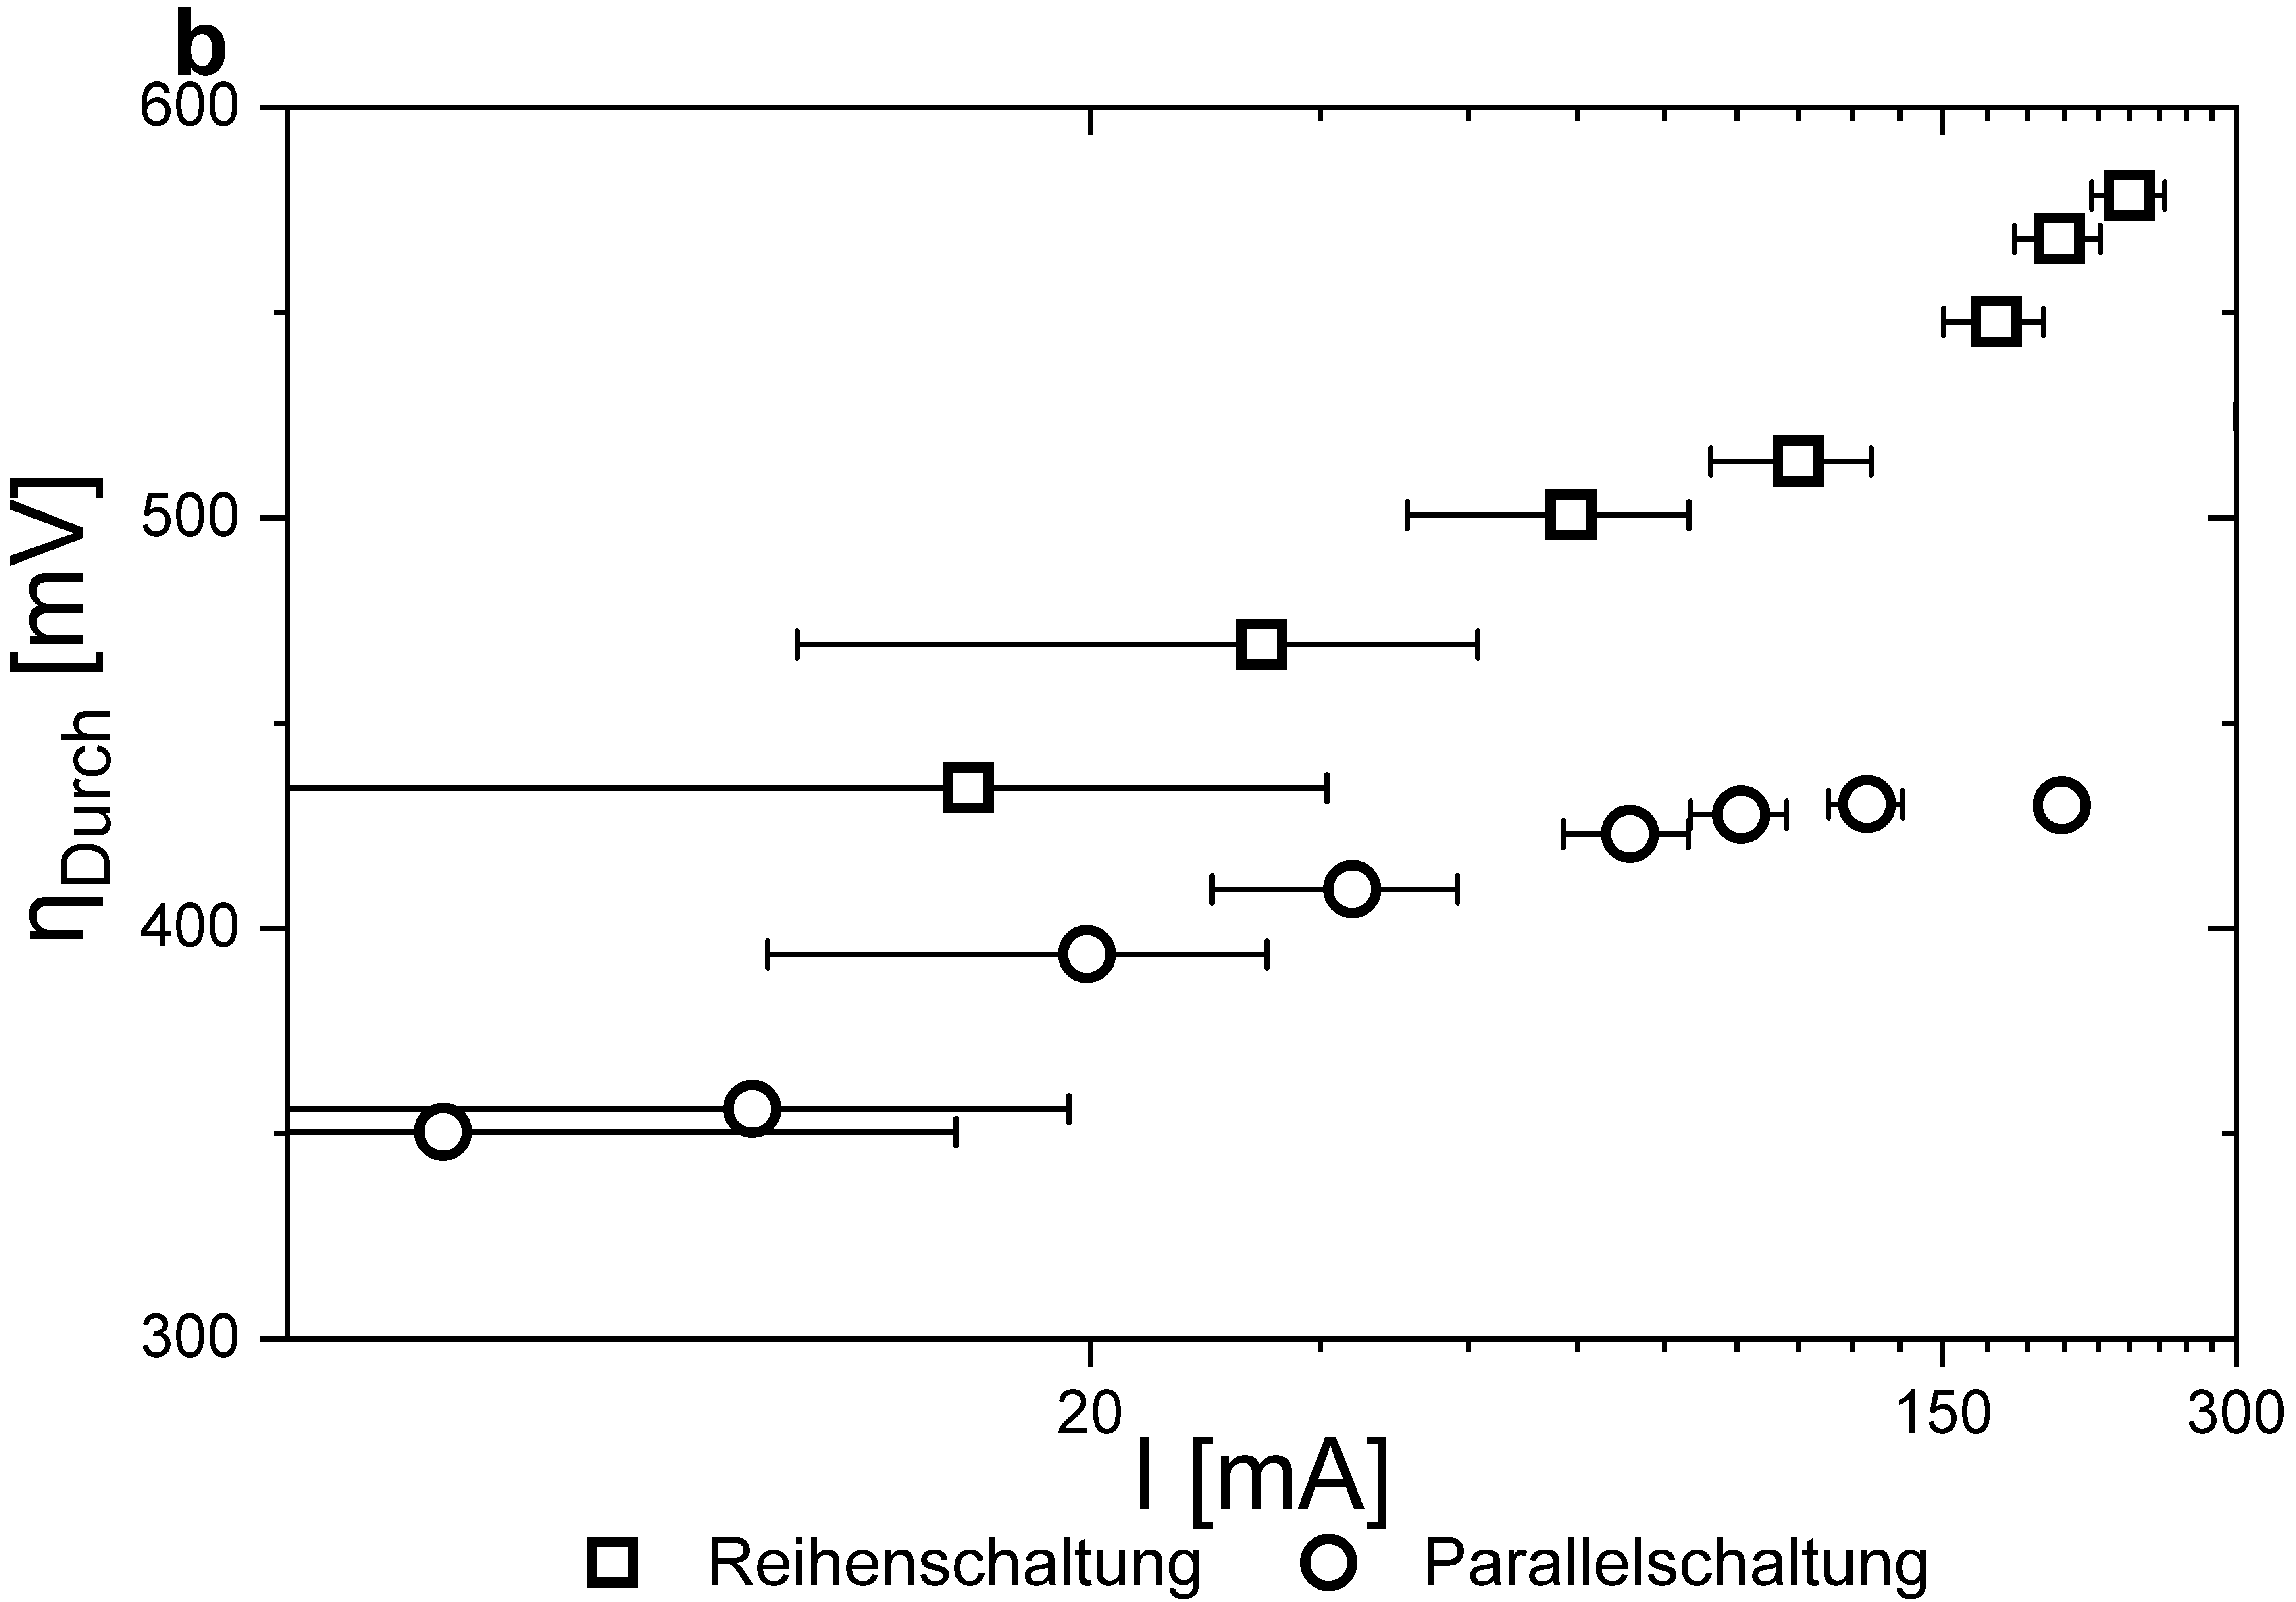
\includegraphics[width=79mm]{graphs/zelleChar1.png}
                    \caption{
                        \textbf{a} Kennlinien einer Brennstoffzelle in Parallel- und Reihenschaltung. Werte links von $I_e$ befinden sich im elektrokinetischen Bereich. Werte rechts von $I_e$ befinden sich im ohmschen Bereich der jeweiligen Kennlinie. Beide Kurven werden für die Berechnung des Innenwiderstands verwendet und stellen nicht konkret den weiteren Verlauf der dargestellten Werte dar.
                        \textbf{b} Berechnete Durchtrittsspannung $\eta_{\mathrm{Durch}}$ jeweiliger aufgenommener Datenpunkte. $\eta_{\mathrm{Durch}}$ wurde mittels Gleichung \ref{eq:etaDurch} berechnet. Man beachte dass nicht alle Datenpunkte dargestellt sind, da sich nur wenige dieser im elektrokinetischen Bereich befinden.\\
                        Aufgrund kleiner Unsicherheiten, sind diese teilweise schwer erkennbar.
                    }
                    \label{fig:brennVerbrauchRate}
                \end{figure*}
        
        
        \subsection{Kennlinie der Brennstoffzelle}\label{subsec:char_brenn}
            In Abbildung \ref{fig:brennVerbrauchRate} sind die Kennlinien der Brennstoffzelle in Parallel- und Reihenschaltung sichtbar. Da die gemessenen Daten sich auf beide Brennstoffzellen beziehen, wurden diese für die Darstellung der Kennlinien auf eine Brennstoffzelle umgerechnet. Es wurde angenommen, dass beide identisch sind. Für die Parallelschaltung wurde die Umrechnung durch folgenden Formeln vorgenommen.
            \begin{center}
                $U_{\mathrm{Messung}} = U_{\mathrm{Zelle,1}} = U_{\mathrm{Zelle,2}} = U_{\mathrm{Zelle}}$
                $I_{\mathrm{Messung}} = I_{\mathrm{Zelle,1}} + I_{\mathrm{Zelle,2}} = 2\cdot I_{\mathrm{Zelle}}$    
            \end{center}
            Für die Reihenschaltung wurden folgenden Formeln verwendet.
            \begin{center}
                $U_{\mathrm{Messung}} = U_{\mathrm{Zelle,1}} + U_{\mathrm{Zelle,2}} = 2\cdot U_{\mathrm{Zelle}}$
                $I_{\mathrm{Messung}} = I_{\mathrm{Zelle,1}} = I_{\mathrm{Zelle,2}} = I_{\mathrm{Zelle}}$  
            \end{center}
            Für die in Kapitel \ref{subsec:char_zel} zu berechnenden Charakteristiken, wird der Innenwiderstand der Brennstoffzelle benötigt. Dieser kann aus dem ohmschen Bereich der Kennlinie bestimmt werden. Aufgrund des nahezu linearen Zusammenhang von Strom zu Spannung, kann dieser unter der Beziehung $\eta_{Ohm} = R_{\mathrm{Innen}} I$ aus der Steigung der jeweiligen Kennlinie bestimmt werden.
            Umstellen liefert $R_{\mathrm{Innen}} = \frac{\eta_{Ohm}}{I}$. Hierbei setzt man $\eta_{Ohm}$ mit $U$ in Abbildung \ref{fig:brennVerbrauchRate} gleich, und liest somit $\frac{U}{I}$ über die Steigung der Ausgleichsgerade ab. Hierbei erhält man eine Steigung von $\mathbf{R_{\mathrm{Innen}} = (2,01 \pm 0,01)} \,\bm{\Omega}$  für die Reihenschaltung und $\mathbf{R_{\mathrm{Innen}} = (1,61 \pm 0,01)}\,\bf{\Omega}$ für die Parallelschaltung. Diese stellen den Innenwiderstand der Brennstoffzelle dar.
            
        
        \subsection{Charakterisierung der Elektrochemischen Zelle}\label{subsec:char_zel}
            Im folgenden soll der Durchtrittsfaktor $\alpha$ und die Austauschstromstärke $I_0$ berechnet werden. Zuerst wurde für alle aufgenommenen Datenpunkte $\eta_{\mathrm{Durch}}$ berechnet, und in Abbildung \ref{fig:brennVerbrauchRate}b dargestellt. Dabei wurden die Datenpunkte auf eine einzelne Brennstoffzelle zurückgerechnet, sowie $R_{\mathrm{Innen}} = 1,61 \Omega$ verwendet.
            \\
            Nun kann durch Abbildung \ref{fig:brennVerbrauchRate}b Funktion \ref{eq:fit} gefittet werden. Werte für $s$ und $v$ sind in Tabelle \ref{tab:fittingVal} dargestellt.
            \begin{table}
                \centering
                \begin{tabular}{c|c|c}
                    \multicolumn{1}{c}{Schaltung} & \multicolumn{1}{c}{$s$} & \multicolumn{1}{c}{$v$}\\
                    \cmidrule(lr){1-1}\cmidrule(lr){2-2}\cmidrule(lr){3-3}
                    \toprule
                    a & (0,028 $\pm$ 0,012) & (0,376 $\pm$ 0,056) \\
                    b & (0,026 $\pm$ 0,021) & (0,30 $\pm$ 0,07) \\
                    \bottomrule
                \end{tabular}
                \caption{Berechnete Parameter \textbf{a} der Reihenschaltung und \textbf{b} der Parallelschaltung.}
                \label{tab:fittingVal}
            \end{table}
            \\
            Unter Verwendung dieser Werte kann nun $\alpha$ und $I_0$ berechnet werden. Hierzu verwendet man Funktion \ref{eq:durchtrittsfaktor}, sowie Funktion \ref{eq:austauschstrom}.
            Für die Reihenschaltung ergeben sich folgende Ergebnisse.
            \begin{center}
                $\mathbf{I_0 = -2,05 \cdot 10^{-6}}$ \textbf{A}    
            \end{center}
            \begin{center}
                $\bm{\alpha}\, \mathbf{ = 0,55} \quad$ . 
            \end{center}
            \\
            Für die Parallelschaltung ergeben sich folgende Ergebnisse.
            \begin{center}
                $\mathbf{I_0 = -7,28 \cdot 10^{-6}}$ \textbf{A}    
            \end{center}
            \begin{center}
                $\bm{\alpha}\, \mathbf{ = 0,51} \quad$ . 
            \end{center}
            
        
        
    \section{Diskussion}\label{sec:discussion}
        \subsection{Charakterisierung des Elektrolyseurs}
            Im folgenden betrachte man Abbildung \ref{fig:leckRate}b. Wie an den ersten drei Datenpunkten gut erkennbar ist, besitzt die Kurve bei einer Spannung von etwa $1,4$ V einen geringen Anstieg. Dies liegt daran, dass für die Elektrolyse von Wasser eine gewisse Spannung benötigt wird. Diese liegt bei etwa $U_{\mathrm{theo}} = 1,23$ V \citep{anleitung}. Da es sich bei dem verwendeten Elektrolyseur nicht um einen idealen Elektrolyseur handelt, wird aufgrund von verschiedenen Verlusten und Einflussfaktoren eine höhere Spannung benötigt. Beginnt die Zersetzung des Wassers, wurde eine gewisse Spannung erreicht, so kann ein Stromfluss beobachtet werden. Der Stromfluss folgt einem linearen Zusammenhang zwischen $I$ und $U$.
        
        
        \subsection{Wirkungsgrad}
            Beide berechneten Werte der Wirkungsgrade des Elektrolyseurs liegen im Bereich von etwa 80\%. Der hohe Energiewirkungsgrad bedeutet, dass der Elektrolyseur effizient Wasserstoff produziert. Der hohe Faraday-Wirkungsgrad ist ein Indiz dafür, dass keine Nebenreaktionen während der Elektrolyse stattgefunden haben. Da die Erzeugungsrate des Elektrolyseurs nur mit $I = 1$ A durchgeführt wurde, kann für andere Ströme keine konkrete Aussage über das Verhalten bei anderen Strömen getroffen werden. Durch den oben genannten linearen Zusammenhang zwischen $I$ und $U$, kann jedoch angenommen werden, dass der Wirkungsgrad nicht weiter ansteigen wird. Infolgedessen kann von einer leicht fallenden Tendenz ausgegangen werden.
            \\
            Die Wirkungsgrade der Brennstoffzelle liegen im Bereich von 20\% - 80\%. Hierbei handelt es sich um realistische Ergebnisse, da im Allgemeinen der Wirkungsgrad im Bereich von 10\% - 60\% liegt. Der hohe Faradaye-Wirkungsgrad lässt darauf schließen, dass keine Nebenreaktionen in der Brennstoffzelle stattgefunden haben.\\
            Vergleicht man den Energiewirkungsgrad von Elektrolyseur und Brennstoffzelle fällt auf, dass der Elektrolyseur deutlich effektiver Wasserstoff produzieren kann als die Brennstoffzelle verbraucht. Dies lässt darauf schließen, dass mehr Energie bei der Elektrolyse verbraucht wird als das über die Brennstoffzelle gewonnen werden kann. 
        
        
        \subsection{Kennlinie der Brennstoffzelle}
            Der Versuch wurde unter normalen Laborbedingungen durchgeführt. Dies ist beim Vergleich zu Literaturwerten sehr wichtig, da die Betriebstemperatur und der Druck unter Umständen auf das Verhalten der Brennstoffzelle große Auswirkungen haben kann. Im Allgemeinen ist somit ein Vergleich nur bedingt möglich. Eine Betrachtung der Kennlinien in Abbildung \ref{fig:brennVerbrauchRate} wirft Ähnlichkeiten zu Literaturwerten auf. Zudem lassen sich diese gut in die drei bekannten Gebiete unterteilen. Datenpunkte links von $I_e$ befinden sich im elektrokinetischen Bereich. Datenpunkte rechts davon im ohmschen Bereich. Ab $\approx 300$ mA ist in der Kennlinie der Reihenschaltung eine leichte Diffusionshemmung erkennbar. Für eine Konkretisierung dieser Aussage sind aber mehr Datenpunkte und höhere Stromstärken nötig.
            \\
            Hierbei wird angemerkt, dass für eine genaue Charakterisierung der Brennstoffzelle eine einfache Betrachtung der Kennlinie nicht ausreicht. Da in lokalen Bereichen der Brennstoffzelle ein unterschiedliches Verhalten möglich ist, sollte auf weitere Verfahren zurückgegriffen werden \citep{membran}.
            \\
            Beide Kennlinien sind sehr ähnlich, was auch in den berechneten Innenwiderstände sichtbar ist. $R_{\mathrm{Innen}}$ stimmt innerhalb der Unsicherheiten für beide Schaltungen überein. Man beachte, dass die dargestellten Datenpunkte auf jeweils eine Zelle zurückgerechnet wurden. Bei offenem Lastwiderstand besitzt die Reihenschaltung somit eine Leerlaufspannung von $U_0 = 1,6$ V. Die Reihenschaltung erreicht somit eine hohe Leerlaufspannung. Aufgrund der geringen Stromstärke birgt diese jedoch nur eine geringe Leistung. Die Parallelschaltung erreicht hingegen bei einer kleineren Spannung mehr Leistung. Im allgemeinen Gebrauch bietet sich somit eine Kombination beider Schaltungen an, um sowohl hohe Spannung als auch hohe Leistung zu erreichen.
            
            
       \subsection{Charakterisierung der Elektrochemischen Zelle}\label{subsec:discuss_char}
            In Abbildung \ref{fig:brennVerbrauchRate}b ist $\eta_{Durch}$ gegen $I$ aufgetragen. Für Werte im elektrokinetischen Bereich ist $\eta_{\mathrm{Durch}}$ groß, sowie positiv. Für sehr kleine Überspannungen vereinfacht sich die Butler-Volmer-Gleichung \citep{anleitung} zu einem proportionalen Zusammenhang zwischen $I$ und $\eta_{\mathrm{Durch}}$. Für große Überspannungen wird der erste Term in der Butler-Volmer-Gleichung sehr klein und kann vernachlässigt werden. Es resultiert ein exponentieller Zusammenhang zwischen $I$ und $\eta_{\mathrm{Durch}}$. Beide Fälle sind in Abbildung \ref{fig:brennVerbrauchRate}b gut sichtbar und bestätigen somit die korrekte Berechnung. Aufgrund der halblogarithmischen Darstellung, bildet die Kurve im zweiten Fall eine Gerade.
            \\
            Aufgrund der ähnlichen Verläufe von $\eta_{\mathrm{Durch}}$ in beiden Schaltungen, kann von einem ähnlichen Ergebnis ausgegangen werden. Dies spiegelt sich in den Ergebnissen in Kapitel \ref{subsec:char_zel} wieder. 
       
       
    \section{Zusammenfassung}\label{sec:conclusion}
            Zusammenfassend lässt sich erkennen, dass der Elektrolyseur, trotz einer Leckrate, einen hohen Energiewirkungsgrad aufweist. Das bedeutet, dass das Verhältnis zwischen erzeugtem Wasserstoff und Sauerstoff und verwendeter Leistung hoch ist. Sieht man sich jedoch den Wirkungsgrad der Brennstoffzelle an, ist dieser ziemlich gering. Gerade mal 20\% des verwendeten Gases kann in Energie umgewandelt werden. Das ist sehr wenig, wenn man bedenkt, dass es sich bei der Elektrolyse von Wasserstoff und Sauerstoff um eine endotherme Reaktion handelt. Es ist also zu vermuten, dass bei der Erzeugung der Gase mehr Energie verwendet wird, als das mit der Brennstoffzelle gewonnen werden kann. \\
            Außerdem entsteht innerhalb der Zelle das Reaktionsprodukt Wasser. Die Zelle muss daher nach gewissen Zeitabständen gespült werden, damit sie nicht überflutet. Dafür wurde das hergestellte Gas verwendet, dass wiederum nicht für die Energieumwandlung genutzt werden konnte.
            Man kann darauf schließen, dass es sich bei der im Versuch verwendeten Brennstoffzelle um ein nicht sehr effizientes Verfahren zur Gewinnung von Energie handelt.

   

    % References
    \bibliographystyle{mnras}
    \bibliography{Ausarbeitung.bib}
    


    % Appendix
    \appendix
    \section{Fehlerrechnung}\label{subsec:fehler}
            Aus der Tabelle \ref{tab:error} können die Unsicherheiten entnommen werden, die für die Fehlerberechnung verwendet wurden. 
            \begin{table}
                \centering
                \begin{tabular}{c|c|c}
                    \multicolumn{1}{c}{Messgröße} & \multicolumn{1}{c}{Einheit} & \multicolumn{1}{c}{Unsicherheit}\\
                    \cmidrule(lr){1-1}\cmidrule(lr){2-2}\cmidrule(lr){3-3}
                    \toprule
                    Strom I & [A] & 0,02  \\
                    Spannung U &[V]    & 0,005 \\
                    Zeit t &[s]        & 1 \\
                    Druck p &[hPa]     & 20 \\
                    Volumen V &[ml]    & 1,5 \\
                    Temperatur T &[K]
                    & 2\\
                    \bottomrule
                \end{tabular}
                \caption{Verwendete Messgrößen mit systematischer Unsicherheit}
                \label{tab:error}
            \end{table}\\
            Die statistische Unsicherheit des gemessenen Stromes und der gemessenen Spannung der Brennstoffzelle in Parallel- und Reihenschaltung mit einem variierbaren Lastwiderstand wurde mit Hilfe der Student-t-Verteilung für 3 Messreihen auf einem Vertrauensniveau von 62,8\% berechnet. Für die Gesamtunsicherheit wurde die statistische und systematische Unsicherheit linear addiert.\\
            Zur Berechnung der systematischen Unsicherheit vom Wirkungsgrad $\epsilon_E$ für die Brennstoffzelle wurde folgende Gleichung verwendet. $\Delta N_{H_2} = 1\cdot 10^{-4}$\,$mol$ ist hierbei die Unsicherheit des Wasserstoffvolumens.\\
            \begin{equation}
                \owncount
                \begin{aligned}
                \Delta\epsilon_E = \left|\Delta U \cdot \frac{I\cdot t}{\Delta H^{0}\cdot N_{H_2}}\right| + \left|\Delta I \cdot \frac{U\cdot t}{\Delta H^0\cdot N_{H_2}}\right| \\
                + \left|\Delta t \cdot \frac{I\cdot U}{\Delta H^0\cdot N_{H_2}}\right| + \left|\Delta N_{H_2} \cdot \frac{U\cdot I\cdot t}{\Delta H^0\cdot N^2_{H_2}}\right|
                \end{aligned}
            \end{equation}\\
            Für den Faraday-Wirkungsgrad muss zuerst die Unsicherheit des pro Zeit umgesetzten Wasserstoffvolumen berechnet werden. Hierfür wurde nachfolgende Formel verwendet.
            \begin{equation}
                \owncount
                \begin{aligned}
                \Delta \dot{V}_{\mathrm{H_2, theo}} = \left|\Delta I \cdot \frac{R\cdot T}{p\cdot z\cdot F}\right| + \left|\Delta T \cdot \frac{I\cdot R}{p\cdot z\cdot F}\right| \\
                +\left|\Delta p \cdot \frac{I\cdot T\cdot R}{p^2\cdot F\cdot z}\right|
                \end{aligned}
                \label{eq:vh2theo}
            \end{equation}\\
            Nun kann der Faraday-Wirkungsgrad berechnet werden. Die Unsicherheit des experimentell bestimmten pro Zeit umgesetzten Wasserstoffvolumen wurde auf \SI{0,01}{\milli\litre} gesetzt. 
            \begin{equation}
            \owncount
            \Delta\epsilon_F = \left|\Delta \dot{V}_{\mathrm{H_2, theo}} \cdot \frac{1}{\dot{V}_{\mathrm{H_2, exp}}}\right|+ \left|\Delta \dot{V}_{\mathrm{H_2, exp}} \cdot \frac{\dot{V}_{\mathrm{H_2, theo}}}{\dot{V}_{\mathrm{H_2, theo}}^2}\right|
            \end{equation} \\
            Der Wirkungsgrad $\epsilon_E$ des Elektrolyseurs wurde folgendermaßen berechnet. Hier ist $\Delta N_{H_2} = 5,5 \cdot 10^{-4}$\,$mol$ die Unsicherheit des Wasserstoffvolumens. 
            \begin{equation}
                \owncount
                \begin{aligned}
                \Delta \epsilon_E = \left|\Delta N_{H_2} \cdot \frac{\Delta H^0}{U\cdot I\cdot t}\right| + \left|\Delta U \cdot \frac{\Delta H^0\cdot N_{H_2}}{U^2\cdot T\cdot t}\right| \\
                +\left|\Delta I \cdot \frac{\Delta H^0 \cdot N_{H_2}}{U\cdot I^2 \cdot t}\right| + \left|\Delta t \cdot \frac{\Delta H^0\cdot N_{H_2}}{U\cdot I\cdot t^2}\right|
                \end{aligned}
            \end{equation}\\
            Zur Berechnung des Faraday-Wirkungsgrads wird die Unsicherheit des pro Zeit umgesetzten Volumens mit der Gleichung \ref{eq:vh2theo} berechnet. Anschließend kann die Unsicherheit des Wirkungsgrads folgendermaßen berechnet werden. 
            \begin{equation}
                \owncount
                \Delta \epsilon_F = \left|\dot{V}_{\mathrm{H_2, exp}}\cdot \frac{1}{\dot{V}_{\mathrm{H_2, theo}}}\right| + \left|\Delta \dot{V}_{\mathrm{H_2, theo}}\cdot\frac{\dot{V}_{\mathrm{H_2, exp}}}{\dot{V}_{\mathrm{H_2, theo}}^2}\right|
            \end{equation}\\
            %Zur Berechnung der Unsicherheiten des Innenwiderstandes der Brennstoffzelle wurde aus der Messreihe über quadratische Addition die statistische Unsicherheit errechnet. Die Formel dafür sieht wie folgt aus.
            %\begin{equation}
                %\owncount
                %\Delta R_{Inn_{stat}} = \sqrt{\Delta U^2\cdot\left(\frac{1}{I}\right)^2 + \Delta I^2\cdot \left(\frac{U}{I^2}\right)^2}
           % \end{equation}\\
            %Für $\Delta U$ und $\Delta I$ wurde jeweils der Mittelwert aus der Messreihe gebildet. Da nur wenige Messwerte vorlagen, wurde dieser mit der Student-t-Verteilung auf einem Vertrauensniveau von 62,8\% ergänzt.\\
            %Die systematische Unsicherheit des Widerstandes lässt sich wie folgt berechnen.
            %\begin{equation}
               % \owncount
                %\Delta R_{Inn_{sys}} = \left|\Delta U \cdot %\frac{1}{I}\right| + \left|\Delta I \cdot \frac{U}{I^2}\right|
            %\end{equation}

        


    \label{lastpage}
\end{document}
